\documentclass[11pt]{article}
\usepackage[a4paper,hscale=0.74,vscale=0.95]{geometry}

%\usepackage[latin1]{inputenc}
%\usepackage{charter}
\usepackage[german,english]{babel}
%\usepackage{url}
%\usepackage{pdfsetup}
\usepackage{eurosym}
\usepackage{graphicx}
\usepackage{verbatim}
%\usepackage{float}
\usepackage{tikz}

\usepackage{xeCJK}
%\setCJKmainfont[BoldFont=STZhongsong, ItalicFont=STKaiti]{STSong}
%\setCJKsansfont[BoldFont=STHeiti]{STXihei}
%\setCJKmonofont{STFangsong}

\parindent 0pt
\parskip 1ex
\begin{document}
\setcounter{tocdepth}{1}

\newcommand{\alert}[1]{{\color{red}{#1}}}

\begin{center}
{\Large\bf A Detailed Travel Guide from Shanghai Pudong Airport to Nanjing}
\end{center}

The benefit of going through Shanghai Pudong International Airport (浦东机场, IATA: PVG) 
is that PVG is one major international airport of China which has more flight choices. 
PVG has two large terminals (T1 and T2) arranged as the verticals of a H shape. 
The crosspiece of the H is a walkway with moving sidewalks and transport connections 
such as airport bus, metro line and the fast Maglev trains (as shown in Fig~\ref{pvg}).

\begin{figure}[h]
	\begin{center}
		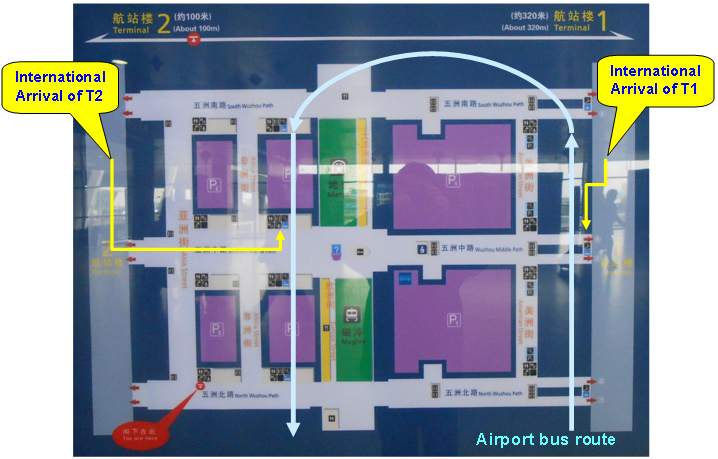
\includegraphics[scale=0.6]{pvg2.jpg}
	\end{center}
 	 \caption{Plan of Shanghai Pudong International Airport.\label{pvg}}
 \end{figure}
 
 The suggested path from PVG is as follows:
 
 \begin{center}
 \begin{tabular}{| l | p{1.5cm} | p{4cm} | p{6cm}|}
  	\hline
	\textbf{Hop} 	&	\bf{From}		& \bf{To	}								& \bf{By} \\
	\hline
	1					&	PVG				& Hongqiao Railway Station (虹桥火车站)	& Airport Bus Line 1, %
	which operates every 15$\sim$25 minutes from 7:00 a.m. to 23:00 p.m. The journey takes about %
	one and half hour. Ticket price is \textyen20. Get off   at Hongqiao Railway (the last stop). %
	Alternatively, you may take metro line 2 and  transfer at GuanLan Road (广兰路) station. \\
	\hline
	2					&	Hongqiao Railway Station 	& Nanjing South Railway Station (南京南站, shown as NanJingNan on the ticket) & High speed train (Gxxx)	\\
	\hline
	3					& Nanjing South Railway Station & Hanyuan Hotel	& Taxi \\			
	\hline
\end{tabular}
\end{center}

\section{Details of Hop 1}

The blue lines in Fig~\ref{pvg}. show the route of airport buses which run on ground floor, connecting T1 and T2. 
International arrival of T1 is on the ground floor. Following the yellow line in Fig 1., going through exit gate 10 (Fig~\ref{pic2}), 
you can get to airport bus stops. Please take Airport Bus Line No.1 (Fig~\ref{pic3}).

\begin{figure}[h]
    \centering
    	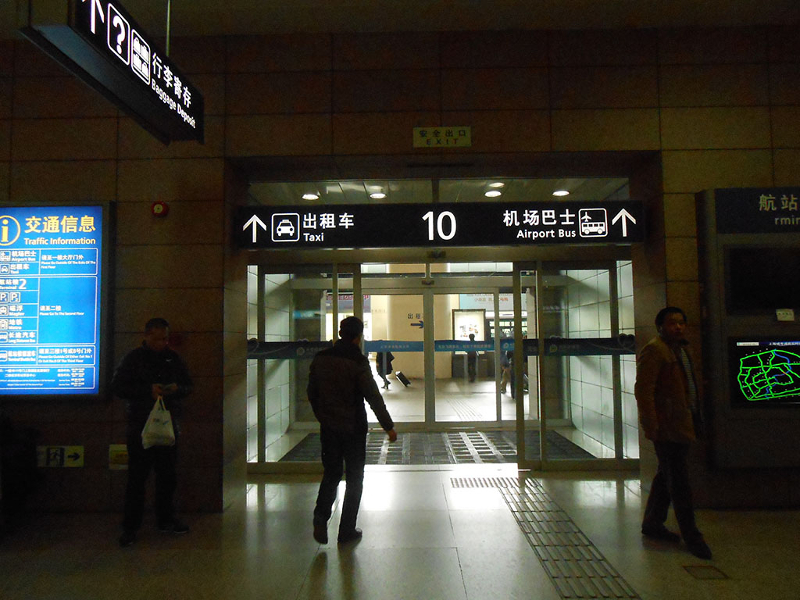
\includegraphics{image003.jpg}
    	\caption{Exit gate 10 of T1.\label{pic2}}
 \end{figure}
		 
\begin{figure}[h]
	\begin{minipage}[t]{.5\textwidth}
     	\centering
        	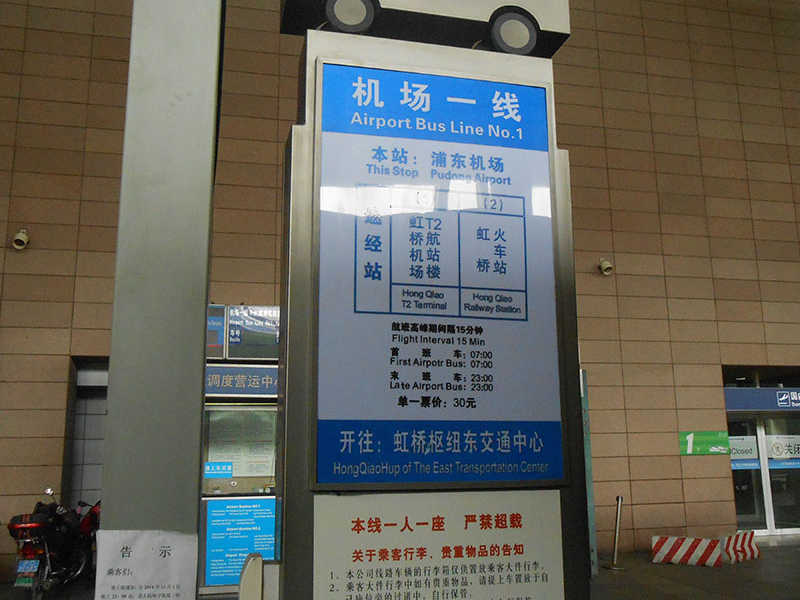
\includegraphics{image005.jpg}
	\end{minipage}%
     \begin{minipage}[t]{.5\textwidth}
         \centering
         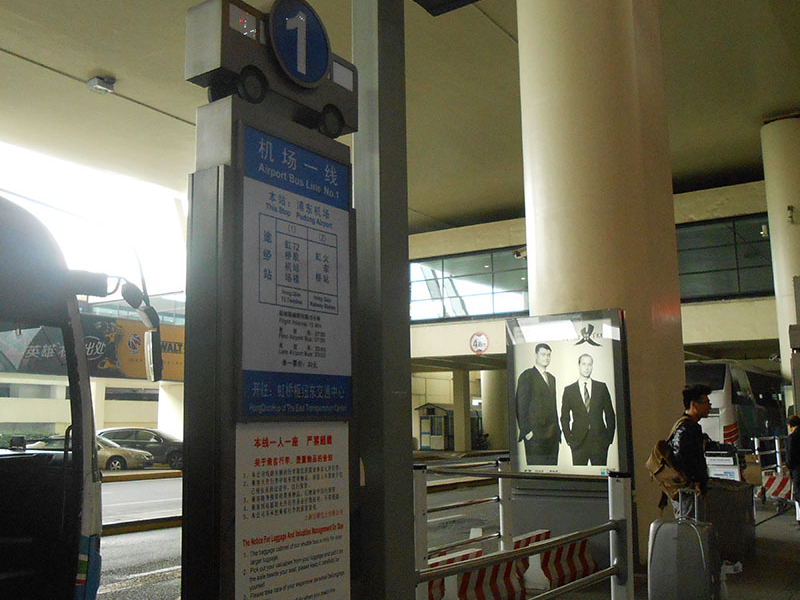
\includegraphics[scale=1.0]{image007.jpg}
    \end{minipage}%
	\caption{Airport Bus Line No. 1 at T1.\label{pic3}}
 \end{figure}
  
 Different from T1, International arrival of T2 is on the first floor. Go alone yellow line (Fig~\ref{pvg}), get onto North Wuzhou Path (Fig~\ref{pic4}), follow the overhead directions, you will reach the gate leading to Airport Bus stops (Fig~\ref{pic5}, Fig~\ref{pic6}). Please take Line No.1 (Fig~\ref{pic7}). 
 \begin{figure}[h]
    \centering
    	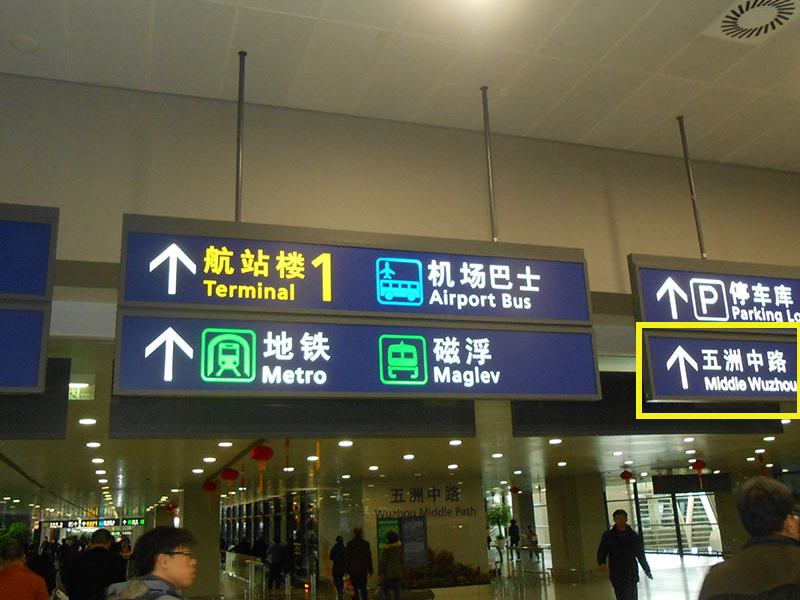
\includegraphics{image010.jpg}
    	\caption{Middle Wuzhou Path.\label{pic4}}
 \end{figure}
\begin{figure}[!h]
	\begin{minipage}[t]{.5\textwidth}
     	\centering
        	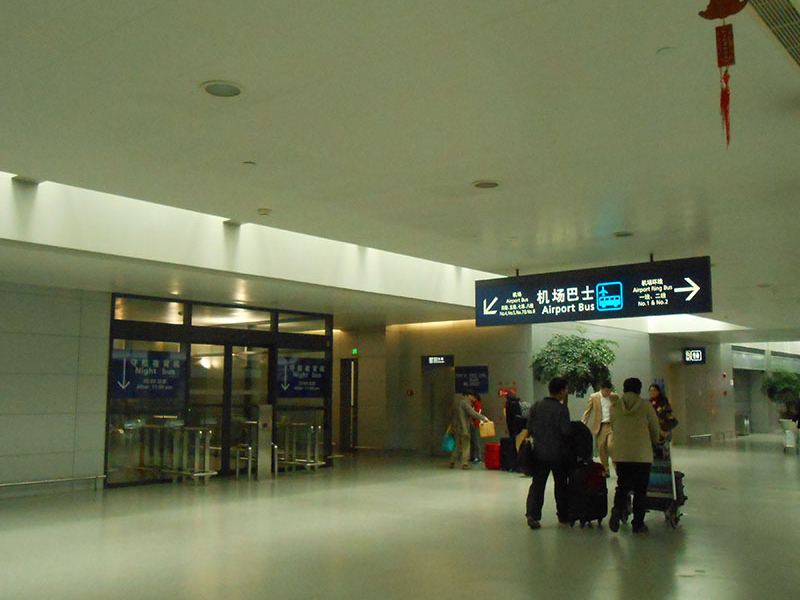
\includegraphics{image012.jpg}
	\end{minipage}%
     \begin{minipage}[t]{.5\textwidth}
         \centering
         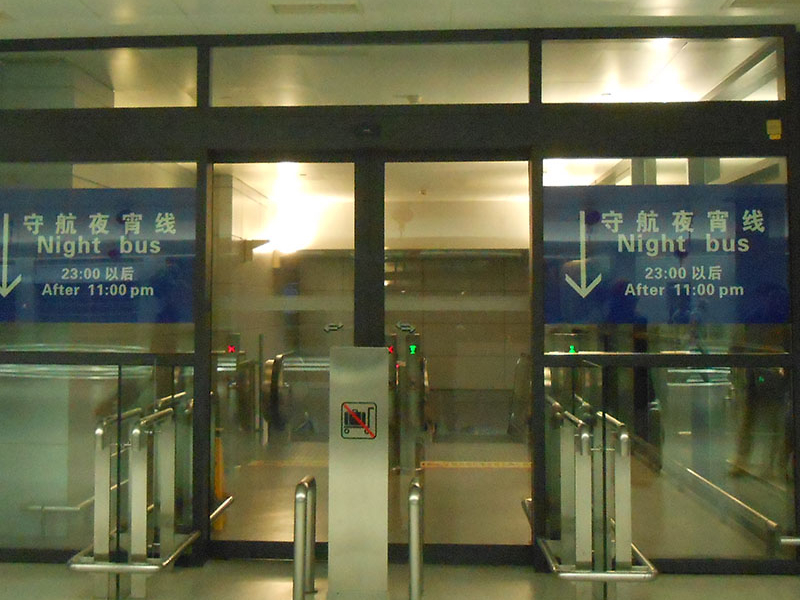
\includegraphics[scale=1.0]{image014.jpg}
    \end{minipage}%
	\caption{The gate leading to Airport Bus stops.\label{pic5}}
 \end{figure}
 \begin{figure}[!h]
    \centering
    	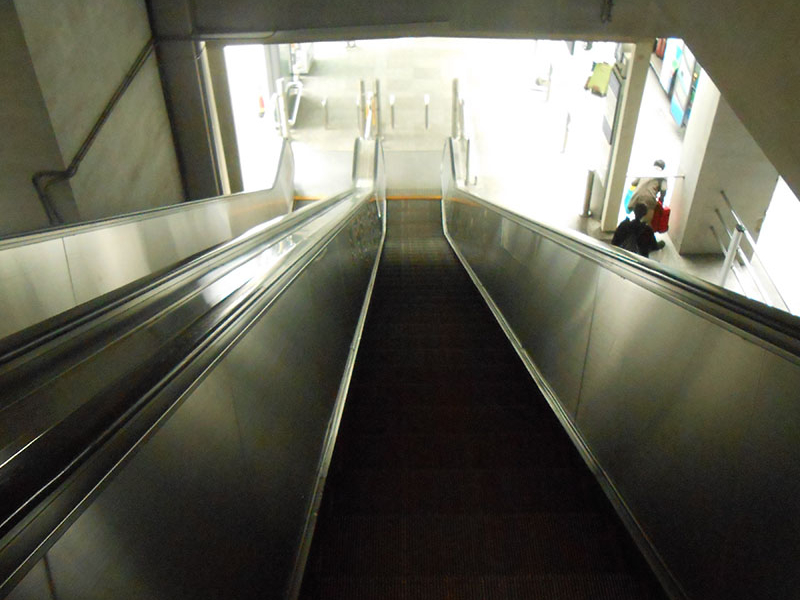
\includegraphics{image016.jpg}
    	\caption{Escalator behind the door.\label{pic6}}
 \end{figure}
\begin{figure}[!h]
	\begin{minipage}[t]{.5\textwidth}
     	\centering
        	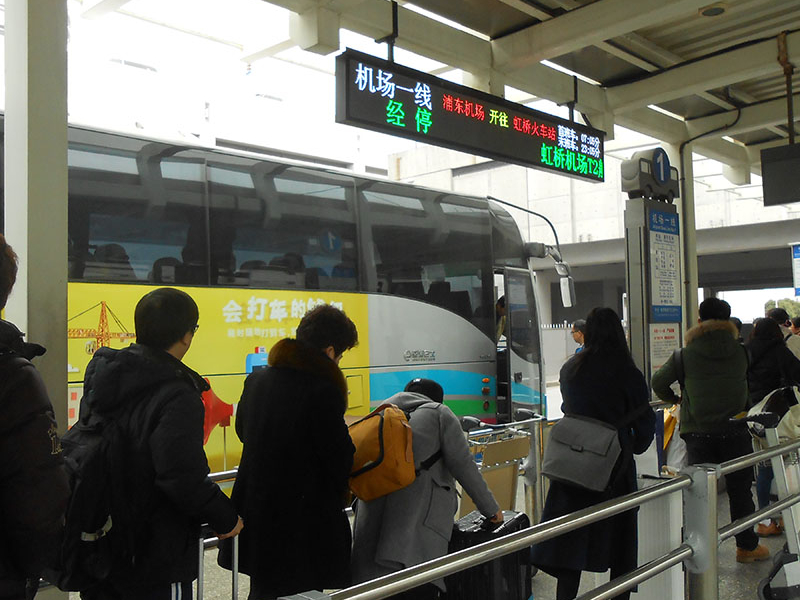
\includegraphics{image018.jpg}
	\end{minipage}%
     \begin{minipage}[t]{.5\textwidth}
         \centering
         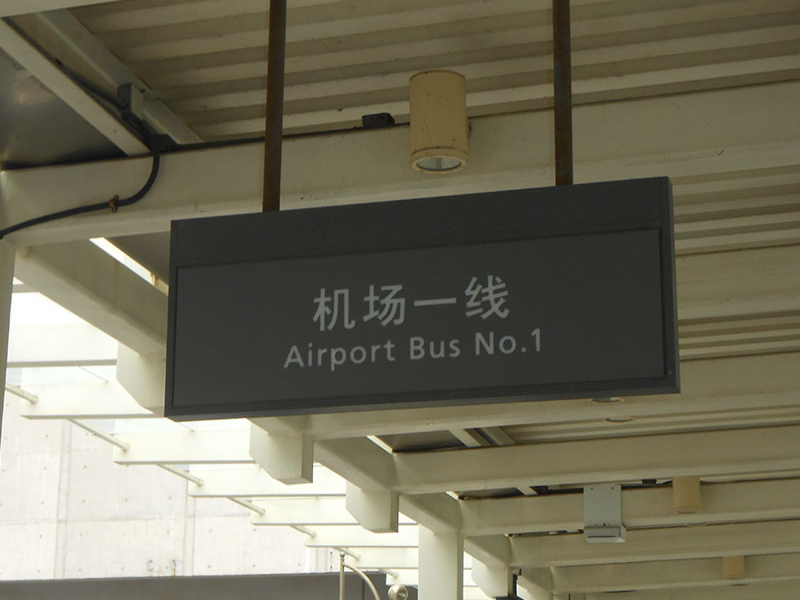
\includegraphics[scale=1.0]{image020.jpg}
    \end{minipage}%
	\caption{The gate leading to Airport Bus stops.\label{pic7}}
 \end{figure}

To go by metro line 2, you need to find the metro station, which locates at the midpoint of Middle Wuzhou Path 
(See Fig~\ref{pvg}). Metro ticket can be bought either from vending machine (Fig~\ref{pic8} shows the button
 for English menu. You need to change for 5 or 10 Yuan notes. There are currency change services nearby 
 the Metro station (see Fig~\ref{pic9}) or international arrivals) or from Metro service center (Fig~\ref{pic10}).
 After transferring at Guanlan Road station, you will reach Hongqiao Railway station. Follow overhead 
 directions (Fig~\ref{pic11}) to get to area A/B which lead to departure floor. You might need to go through 
 a long hallway (Fig~\ref{pic12}) and get to the escalator (Fig~\ref{pic13}) leading to departure floor,
  after which you just need to follow the guides as if you arrive by Airport Bus.
  
\begin{figure}[!h]
	\begin{minipage}[t]{.5\textwidth}
     	\centering
        	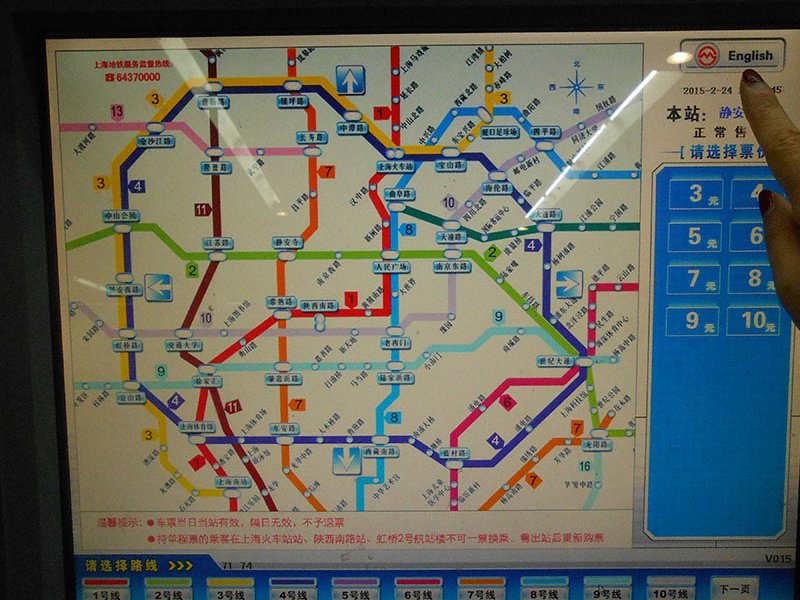
\includegraphics{image022.jpg}
		\caption{Metro ticket vending machine.\label{pic8}}
	\end{minipage}%
     \begin{minipage}[t]{.5\textwidth}
         \centering
         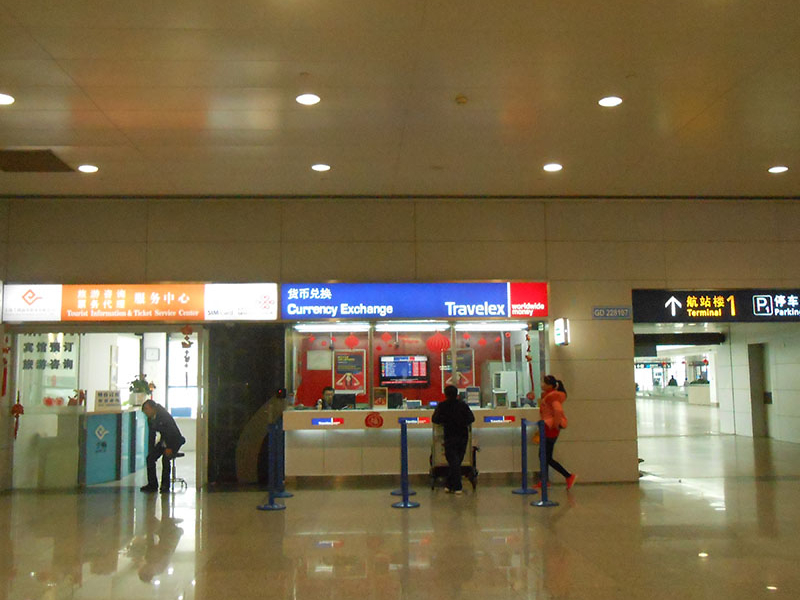
\includegraphics{image026.jpg}
		\caption{Currency change. \label{pic9}}
    \end{minipage}%
 \end{figure}
 
 \begin{figure}[!h]
	\begin{minipage}[t]{.5\textwidth}
     	\centering
        	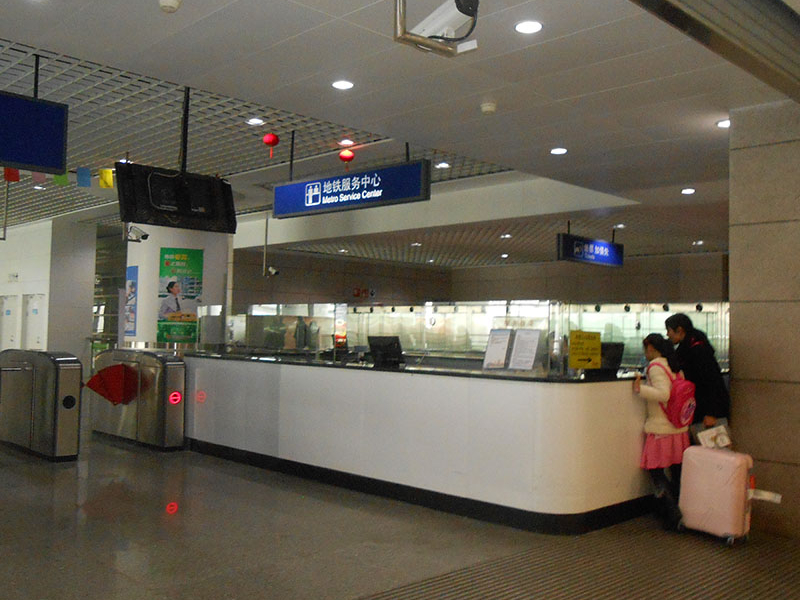
\includegraphics{image024.jpg}
		\caption{Metro service center.\label{pic10}}
	\end{minipage}%
     \begin{minipage}[t]{.5\textwidth}
         \centering
         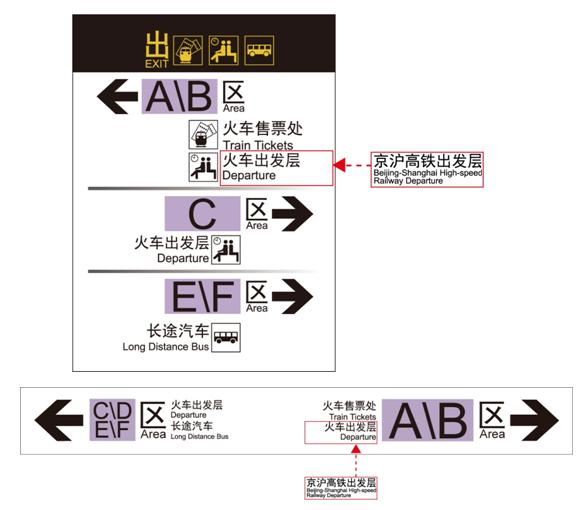
\includegraphics[scale=0.5]{image028.jpg}
		\caption{Directions to area A\slash B.\label{pic11}}
    \end{minipage}%
 \end{figure}
 
  \begin{figure}[!h]
    \centering
    	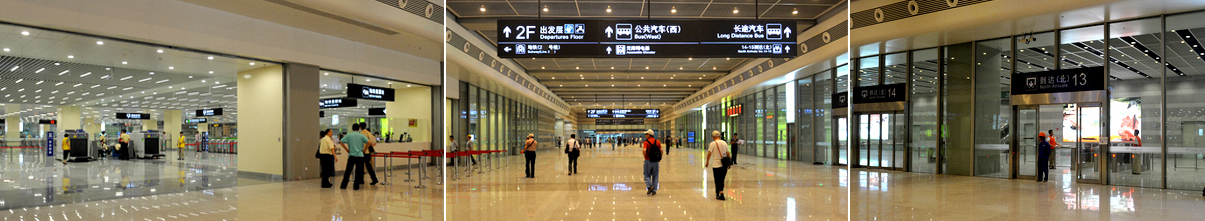
\includegraphics[scale=1.5]{image030.jpg}
    	\caption{Long hallway at area A/B. \label{pic12}}
 \end{figure}
   \begin{figure}[!h]
    \centering
    	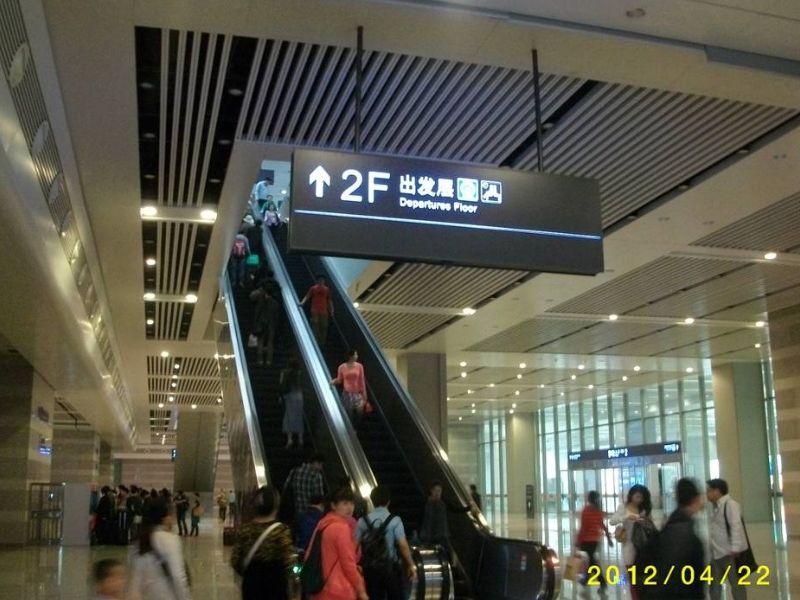
\includegraphics{image032.jpg}
    	\caption{Escalator leading the departure floor. \label{pic13}}
 \end{figure}
  
\newpage
\section{Details of Hop 2}

Airport Bus No. Line 1 goes straight to the South Departure gate of Hongqiao Railway Station (Fig~\ref{pic14}). First, you need to go through the security checking (Fig~\ref{pic15}) to reach the lounge. There are several ticket offices inside the lounge where you can buy a ticket by showing passport (Fig~\ref{pic16}). The formal destination is NanJingNan (南京南, Nanjing South Railway Station).
\begin{figure}[!h]
	\begin{minipage}[t]{.5\textwidth}
     	\centering
        	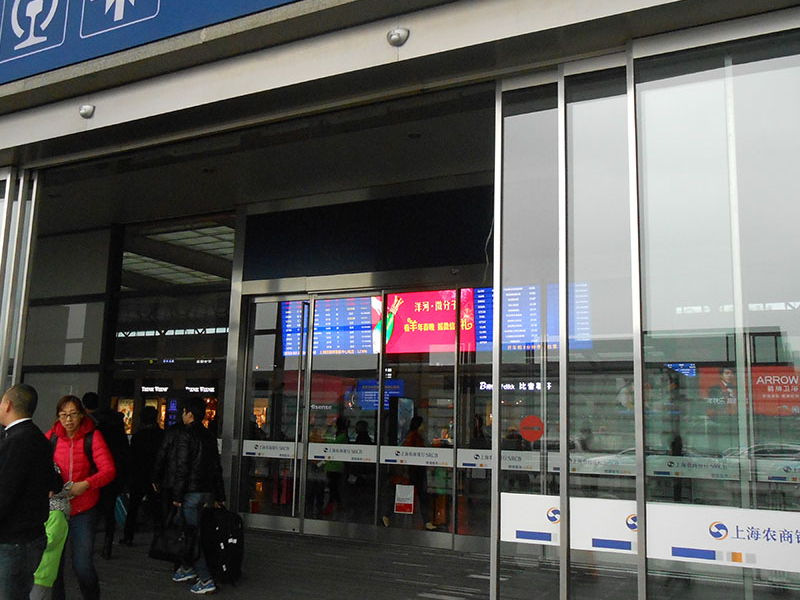
\includegraphics{image034.jpg}
		\caption{South Departure gate. \label{pic14}}
	\end{minipage}%
     \begin{minipage}[t]{.5\textwidth}
         \centering
         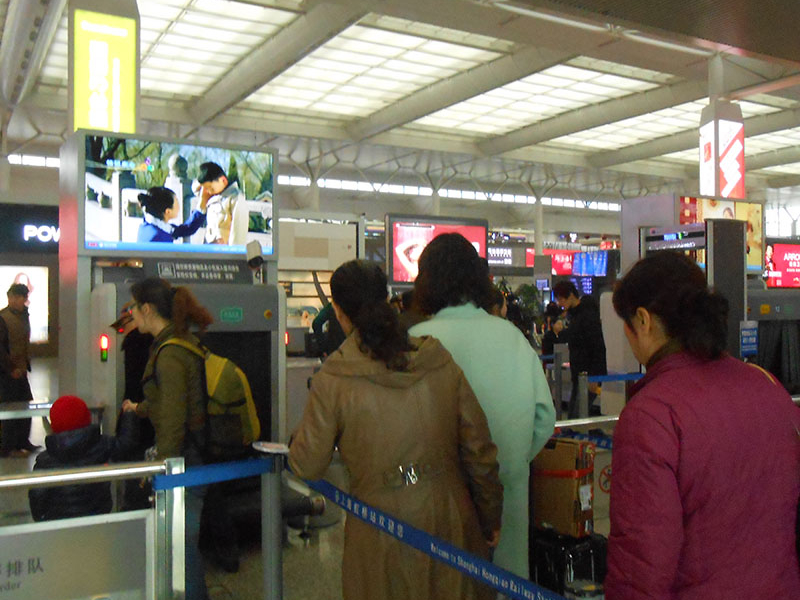
\includegraphics{image036.jpg}  
		\caption{Security Checking. \label{pic15}}
    \end{minipage}%
 \end{figure}
		
\begin{figure}[!h]
	\begin{minipage}[t]{.5\textwidth}
     	\centering
        	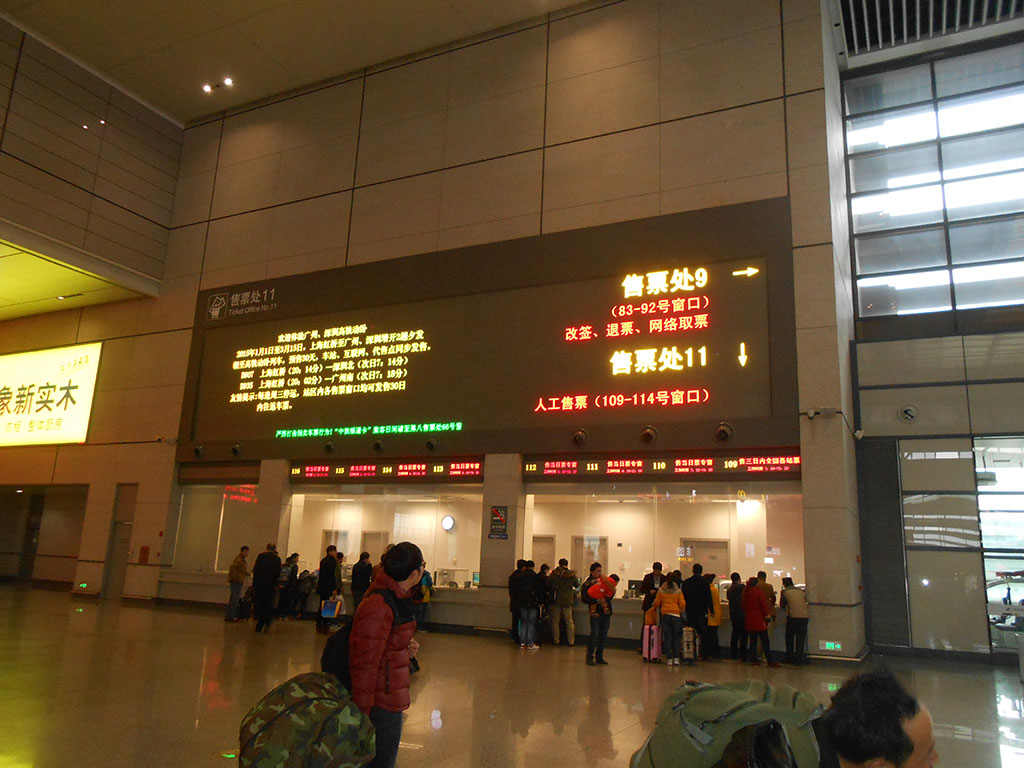
\includegraphics[scale=0.8]{image038.jpg}
	\end{minipage}%
     \begin{minipage}[t]{.5\textwidth}
         \centering
         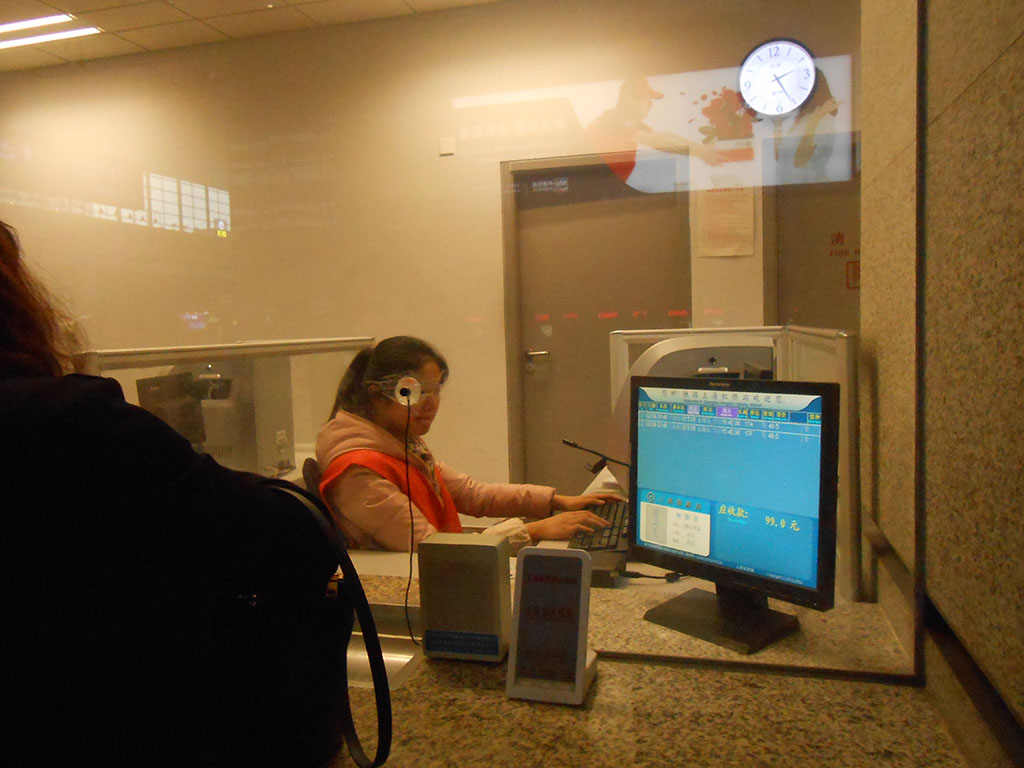
\includegraphics[scale=0.8]{image040.jpg} 
    \end{minipage}%
	\caption{Ticket office inside the lounge.\label{pic16}}
 \end{figure}

Find out the train number and boarding gate on the ticket (Fig\ref{pic17}). Boarding gates can be located easily because there are very clear signs on each of them (Fig\ref{pic18}). 	
\begin{figure}[!h]
	\begin{minipage}[t]{.5\textwidth}
		\hspace{3mm}
		\begin{tikzpicture}
			\node[anchor=south west,inner sep=0] (image) at (0,0) {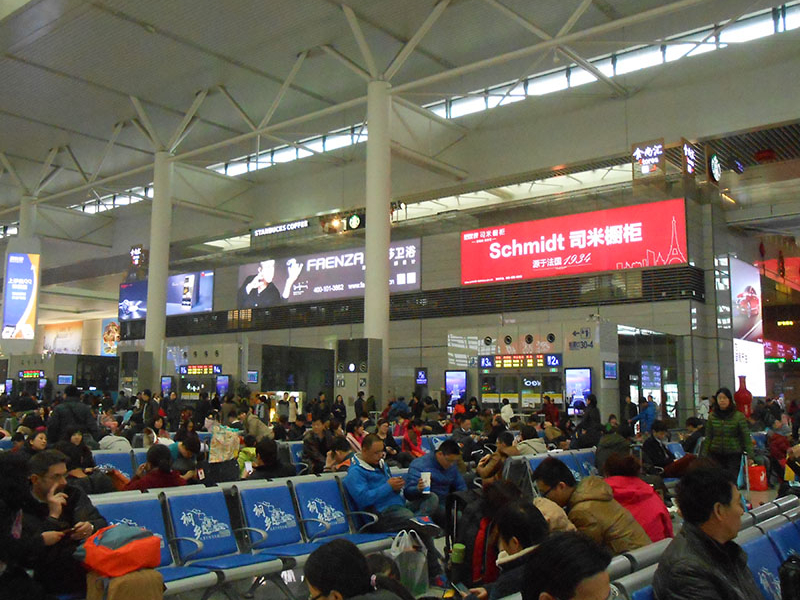
\includegraphics{image043.jpg}}; 
			\begin{scope}[x={(image.south east)},y={(image.north west)}]
				% 建立相对坐标系
				%\draw[help lines,xstep=.1,ystep=.1] (0,0) grid (1,1);
				%\foreach \x in {0,1,...,9} { \node [anchor=north] at (\x/10,0) {0.\x}; }
				%\foreach \y in {0,1,...,9} { \node [anchor=east] at (0,\y/10) {0.\y}; }
				% 作图命令
				\draw [color = yellow!80, ultra thick] (0.52,0.32) rectangle (0.78,0.5);
				\node [anchor=south west,fill=white] at (0.1,0.6) {\bf{Boarding Gate}};
				\draw [->, color = yellow!80, ultra thick] (0.3,0.6) -- (0.52,0.5);
			\end{scope}
		\end{tikzpicture}		
	\end{minipage}%
     \begin{minipage}[t]{.5\textwidth}
         \centering
         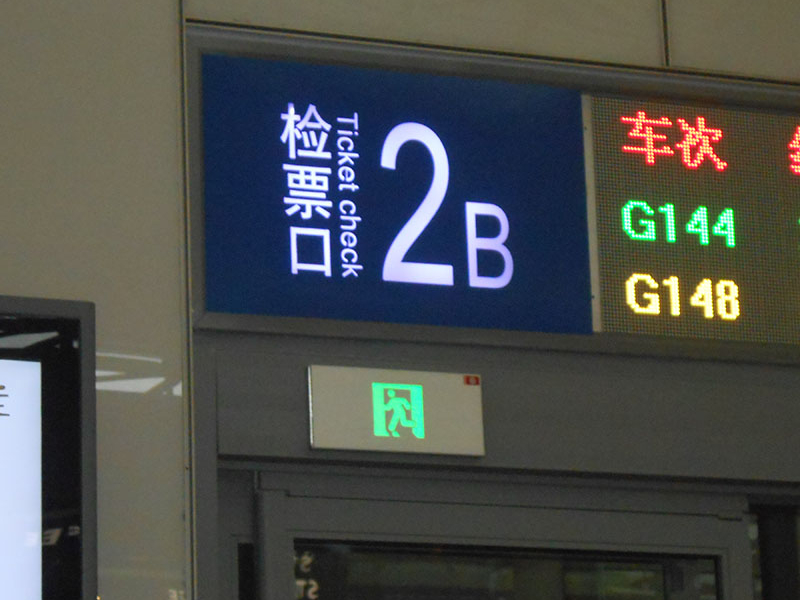
\includegraphics{image046.jpg}
    \end{minipage}%
	\caption{Boarding gate inside the lounge. \label{pic17}}
 \end{figure}

\begin{figure}[!h]
	\centering
	\begin{tikzpicture}
		\node[anchor=south west,inner sep=0] (image) at (0,0) {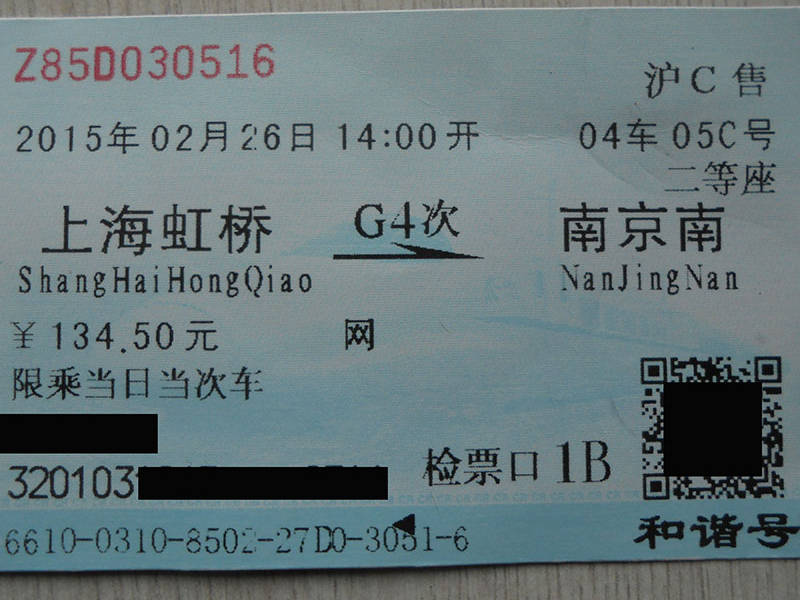
\includegraphics[scale=1.3]{image050.jpg}}; 
		\begin{scope}[x={(image.south east)},y={(image.north west)}]
			% 建立相对坐标系
			%\draw[help lines,xstep=.1,ystep=.1] (0,0) grid (1,1);
			%\foreach \x in {0,1,...,9} { \node [anchor=north] at (\x/10,0) {0.\x}; }
			%\foreach \y in {0,1,...,9} { \node [anchor=east] at (0,\y/10) {0.\y}; }
			% 作图命令
			\draw [color = yellow!80, ultra thick] (0.4,0.55) rectangle (0.61,0.7);
				\node [anchor=south west,fill=white,draw=yellow!80] at (0,0.8) {\bf{Train Number: \alert{G4}}};
				\draw [->, color = yellow!80, ultra thick] (0.3,0.8) -- (0.4,0.7);
				
			\draw [color = yellow!80, ultra thick] (0.7,0.73) rectangle (0.98,0.82);
				\node [anchor=south west,fill=white,draw=yellow!80] at (0.4,0.92) {\bf{Carriage: \alert{04} \ Seat: \alert{05C}}};
				\draw [->, color = yellow!80, ultra thick] (0.6,0.92) -- (0.7,0.82);
				
			\draw [color = yellow!80, ultra thick] (0.5,0.17) rectangle (0.79,0.29);
				\node [anchor=south west,fill=white,draw=yellow!80] at (0.35,0.37) {\bf{Boarding Gate: \alert{1B}}};
				\draw [->, color = yellow!80, ultra thick] (0.6,0.37) -- (0.65,0.29);				
		\end{scope}
	\end{tikzpicture}
	\caption{Reading of a train ticket. \label{pic18}}
\end{figure}

\clearpage

\section{Details of Hop 3}
Get off at South Nanjing railway station, get a taxi and show driver the address of Hanyuan Hotel:

\begin{center}
	 司机师傅,请将我送往``{\bf 童卫路20号翰苑宾馆}'',其位置如地图中红色A点所示。\\
	 酒店电话:02584393962。谢谢!\\ \vspace{5mm}
     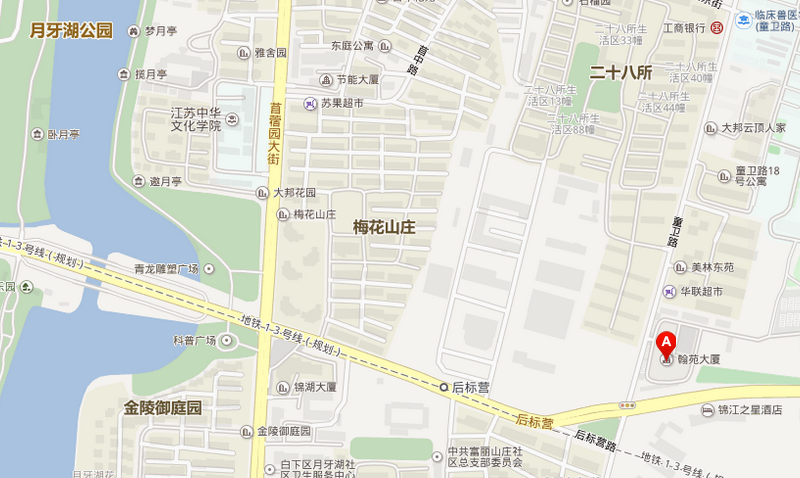
\includegraphics[scale=0.5]{badu.png}
\end{center}

The following figures show how to get to the taxi stop by following overhead directions. 
\begin{figure}[!h]
	\begin{minipage}[t]{.5\textwidth}
     	\centering
        	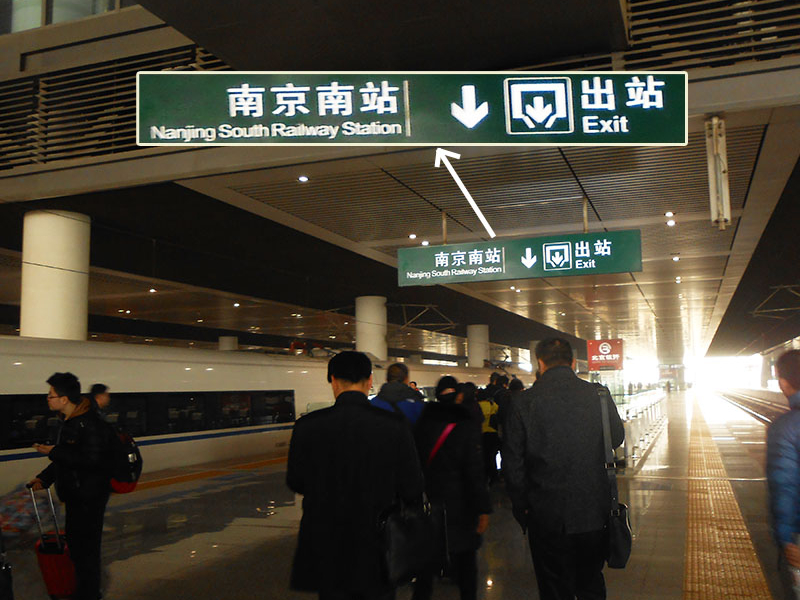
\includegraphics{image053.jpg}
		\caption{Get off the train and go to the exit.}
	\end{minipage}%
     \begin{minipage}[t]{.5\textwidth}
         \centering
         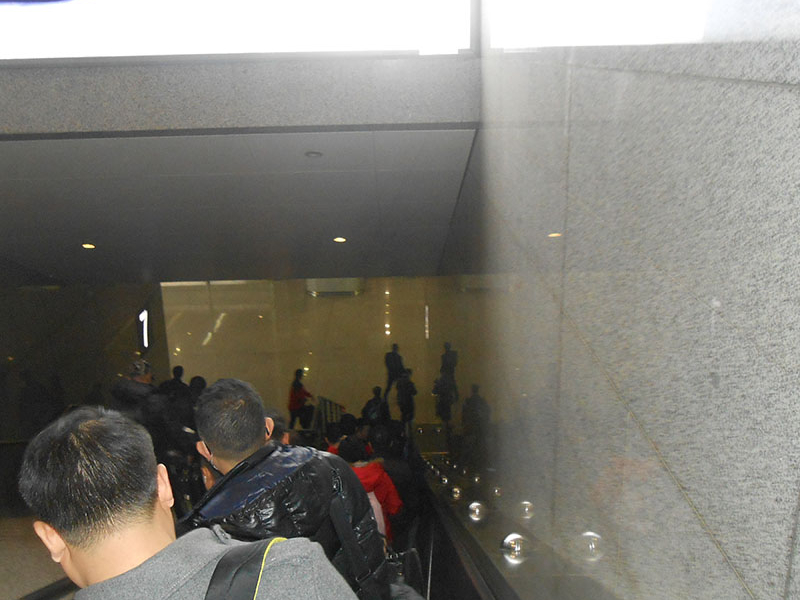
\includegraphics{image055.jpg}
		\caption{Go downstairs via escalator.}
    \end{minipage}%
 \end{figure}

\begin{figure}[!h]
	\begin{minipage}[t]{.5\textwidth}
         \centering
         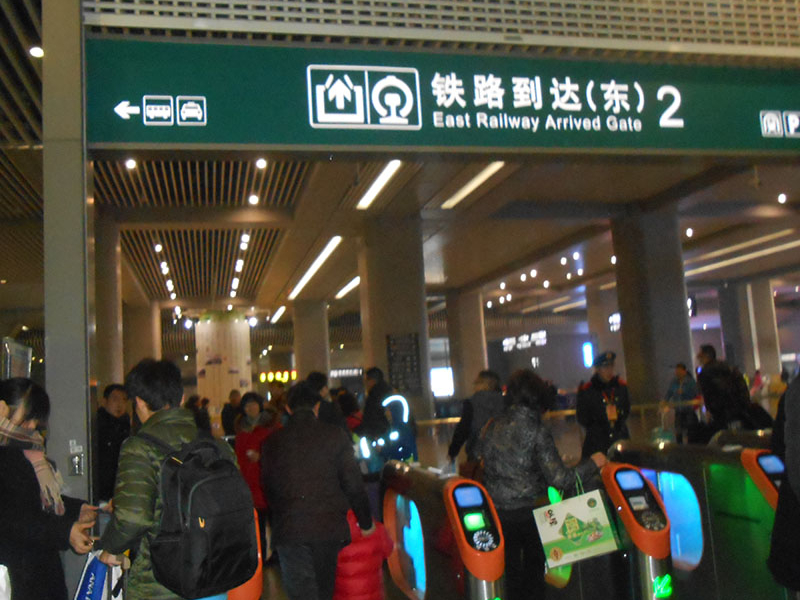
\includegraphics{image057.jpg}
		\caption{Go through the ticket check.}
    \end{minipage}%
	\begin{minipage}[t]{.5\textwidth}
		\hspace{3mm}
		\begin{tikzpicture}
			\node[anchor=south west,inner sep=0] (image) at (0,0) {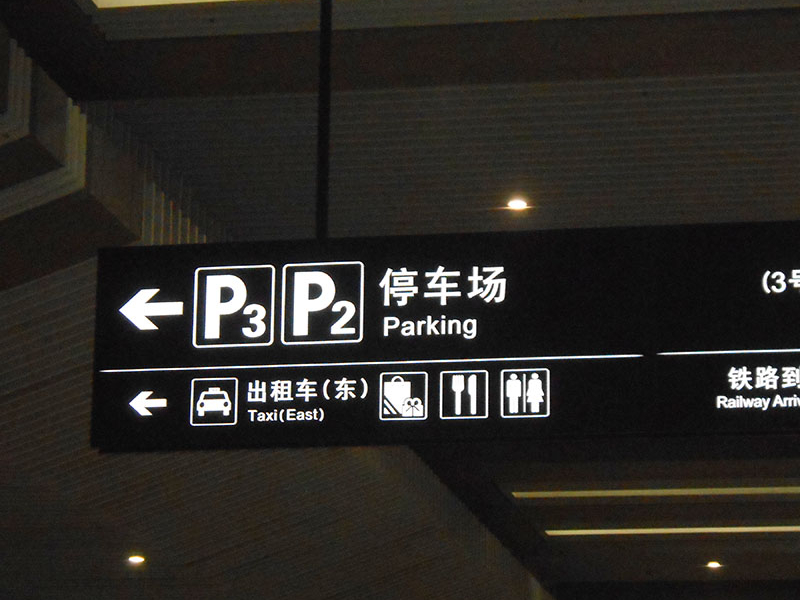
\includegraphics{image060.jpg}}; 
			\begin{scope}[x={(image.south east)},y={(image.north west)}]
				% 建立相对坐标系
				%\draw[help lines,xstep=.1,ystep=.1] (0,0) grid (1,1);
				%\foreach \x in {0,1,...,9} { \node [anchor=north] at (\x/10,0) {0.\x}; }
				%\foreach \y in {0,1,...,9} { \node [anchor=east] at (0,\y/10) {0.\y}; }
				% 作图命令
				\draw [color = yellow!80, ultra thick] (0.2,0.25) rectangle (0.5,0.4);
			\end{scope}
		\end{tikzpicture}		
		\caption{Follow the overhead directions for Taxi (East).}
	\end{minipage}%
 \end{figure}
		
\begin{figure}[!h]
	\begin{minipage}[t]{.5\textwidth}
		\hspace{3mm}
		\begin{tikzpicture}
			\node[anchor=south west,inner sep=0] (image) at (0,0) {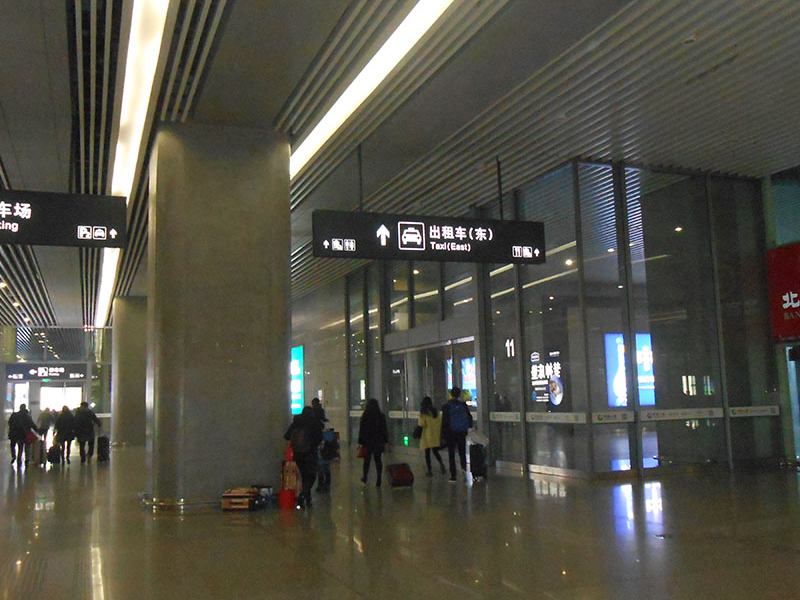
\includegraphics{image063.jpg}}; 
			\begin{scope}[x={(image.south east)},y={(image.north west)}]
				% 建立相对坐标系
				%\draw[help lines,xstep=.1,ystep=.1] (0,0) grid (1,1);
				%\foreach \x in {0,1,...,9} { \node [anchor=north] at (\x/10,0) {0.\x}; }
				%\foreach \y in {0,1,...,9} { \node [anchor=east] at (0,\y/10) {0.\y}; }
				% 作图命令
				\draw [->, color = yellow!80, ultra thick] (0.7,0.1) -- (0.4,0.3);
			\end{scope}
		\end{tikzpicture}		
         \caption{Go through the ticket check.}
    \end{minipage}%
	\begin{minipage}[t]{.5\textwidth}
		\hspace{3mm}
		\begin{tikzpicture}
			\node[anchor=south west,inner sep=0] (image) at (0,0) {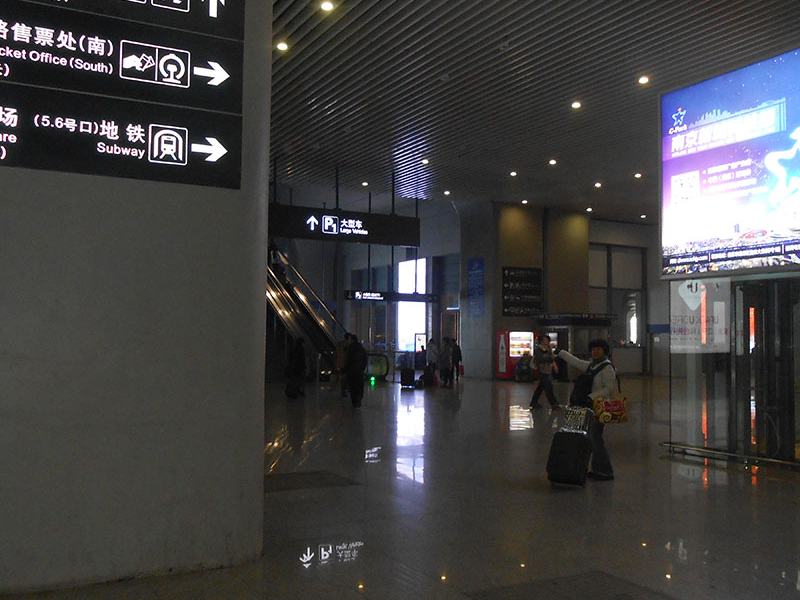
\includegraphics{image069.jpg}}; 
			\begin{scope}[x={(image.south east)},y={(image.north west)}]
				% 建立相对坐标系
				%\draw[help lines,xstep=.1,ystep=.1] (0,0) grid (1,1);
				%\foreach \x in {0,1,...,9} { \node [anchor=north] at (\x/10,0) {0.\x}; }
				%\foreach \y in {0,1,...,9} { \node [anchor=east] at (0,\y/10) {0.\y}; }
				% 作图命令
				\draw [color = yellow!80, ultra thick] (0.45,0.18) rectangle (0.6,0.7);
			\end{scope}
		\end{tikzpicture}		
		\caption{Follow the overhead directions for Taxi (East).}
	\end{minipage}%
 \end{figure}

\begin{figure}[!h]
	\begin{minipage}[t]{.5\textwidth}
		\hspace{3mm}
		\begin{tikzpicture}
			\node[anchor=south west,inner sep=0] (image) at (0,0) {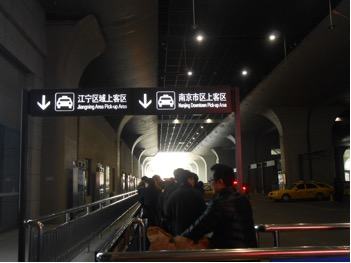
\includegraphics[scale=0.557]{image072.jpg}}; 
			\begin{scope}[x={(image.south east)},y={(image.north west)}]
				% 建立相对坐标系
				%\draw[help lines,xstep=.1,ystep=.1] (0,0) grid (1,1);
				%\foreach \x in {0,1,...,9} { \node [anchor=north] at (\x/10,0) {0.\x}; }
				%\foreach \y in {0,1,...,9} { \node [anchor=east] at (0,\y/10) {0.\y}; }
				% 作图命令
				\draw [color = yellow!80, ultra thick] (0.4,0.55) rectangle (0.68,0.68);
			\end{scope}
		\end{tikzpicture}		
	\end{minipage}%
     \begin{minipage}[t]{.5\textwidth}
         \centering
         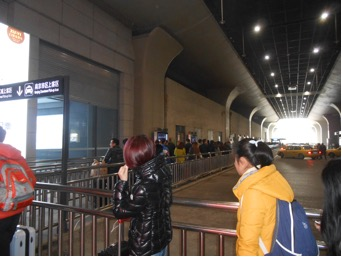
\includegraphics[scale=0.568]{image070.jpg}
    \end{minipage}%
	\caption{Get into the waiting lane for ''Nanjing Downtown'' (less than 20 minutes).}
 \end{figure}

\end{document}